% LaTeX fragment for the PyFock Supporting Information.
% Required packages: \usepackage{graphicx,booktabs}
% The figure paths below assume compilation from this Dynamic_Precision directory.
% If the SI is compiled elsewhere, adjust the two \includegraphics paths accordingly.

\section{Effect of Dynamic Precision on XC Timings}
\label{sec:dynamic_precision_xc}

To quantify the effect of dynamic precision on the exchange--correlation (XC)
evaluation, DFT calculations were performed for
$(\mathrm{H_2O})_{10}$, $(\mathrm{H_2O})_{20}$,
$(\mathrm{H_2O})_{32}$, and $(\mathrm{H_2O})_{47}$ in Kaggle notebook
sessions using a single NVIDIA Tesla T4 or Tesla P100 GPU.  Three independent
notebook runs were carried out for each GPU, with the
\texttt{dynamic\_precision=False} and \texttt{dynamic\_precision=True}
calculations treated as a pair within each run.  Each precision mode was
preceded by an $(\mathrm{H_2O})_{5}$ warm-up calculation to reduce
first-call/JIT overhead; the warm-up calculations were excluded from the
reported data.

All calculations employed PBE/def2-SVP with the def2-universal-jfit auxiliary
basis, an XC block size of 20,480 points, four Numba/BLAS threads, an SCF
energy-convergence threshold of $10^{-7}\ E_{\mathrm h}$, and a maximum of 50
SCF iterations.  PySCF-generated atom-centered quadrature grids were used
(\texttt{use\_pyscf\_grids=True}) at grid level 3.  After pruning, the grids
contained 290,210, 560,702, 884,616, and 1,287,189 points for the four clusters,
respectively.  AO values were recomputed rather than stored
(\texttt{save\_ao\_values=False}).  Dynamic-precision calculations used fp32
in the early SCF iterations and switched to fp64 when the relative change in
the total energy fell below $5\times10^{-6}$ a.u., as described in the main
text.  The switch occurred at iterations 17, 17, 22, and 20 on the T4 and at
iterations 17, 17, 22, and 19 on the P100 for
$(\mathrm{H_2O})_{10}$ through $(\mathrm{H_2O})_{47}$, respectively; these
switch points were identical in all three runs.

The Kaggle sessions used Linux 6.12.90+ (Kaggle Docker image 28755), an
Intel Xeon CPU at 2.00 GHz (2 cores/4 threads), and 31.35 GB host memory.
The benchmark-specific software environment comprised Python 3.12.13,
PyFock 0.1.4, NumPy 2.0.2, SciPy 1.16.3, Numba 0.60.0, llvmlite 0.43.0,
PySCF 2.14.0, numgrid 2.1.2, h5py 3.16.0, Joblib 1.5.3, NumExpr 2.14.1,
opt\_einsum 3.4.0, threadpoolctl 3.6.0, psutil 5.9.5, and
setuptools 81.0.0.

\subsection{Convergence-adjusted timing metric}

A conventional XC time per iteration,
$T_{\mathrm{XC}}/N_{\mathrm{SCF}}$, measures the cost of the iterations that
were actually performed but does not retain the penalty from any additional
SCF iterations introduced by dynamic precision.  We therefore used the
dynamic-off iteration count as a common denominator for each paired run:
\begin{align}
t_{\mathrm{XC,off}}^{\mathrm{eff}}
  &= \frac{T_{\mathrm{XC,off}}}{N_{\mathrm{off}}}, &
t_{\mathrm{XC,on}}^{\mathrm{eff}}
  &= \frac{T_{\mathrm{XC,on}}}{N_{\mathrm{off}}}, \\
S_{\mathrm{XC}}^{\mathrm{eff}}
  &= \frac{t_{\mathrm{XC,off}}^{\mathrm{eff}}}
           {t_{\mathrm{XC,on}}^{\mathrm{eff}}}
   = \frac{T_{\mathrm{XC,off}}}{T_{\mathrm{XC,on}}}.
\end{align}
Equivalently,
\begin{equation}
S_{\mathrm{XC}}^{\mathrm{eff}}
=
\frac{
  (T_{\mathrm{XC,off}}/N_{\mathrm{off}})
  /(T_{\mathrm{XC,on}}/N_{\mathrm{on}})
}{
  N_{\mathrm{on}}/N_{\mathrm{off}}
},
\end{equation}
so the intrinsic per-cycle XC acceleration is explicitly corrected by the
SCF iteration-count factor.  Thus, extra cycles reduce the effective speedup,
whereas fewer cycles increase it.  The bars in
Figures~\ref{fig:dynamic_precision_t4} and
\ref{fig:dynamic_precision_p100} are the arithmetic means of the three paired
run values, and the error bars show one sample standard deviation.  Because
any end-to-end SCF timing remains dependent on the starting density and
convergence path, comparisons are made only within the paired calculations
under the identical protocol stated above.  Total wall times are reported for
completeness but are not interpreted as isolated XC-kernel timings.

\begin{figure}[htbp]
  \centering
  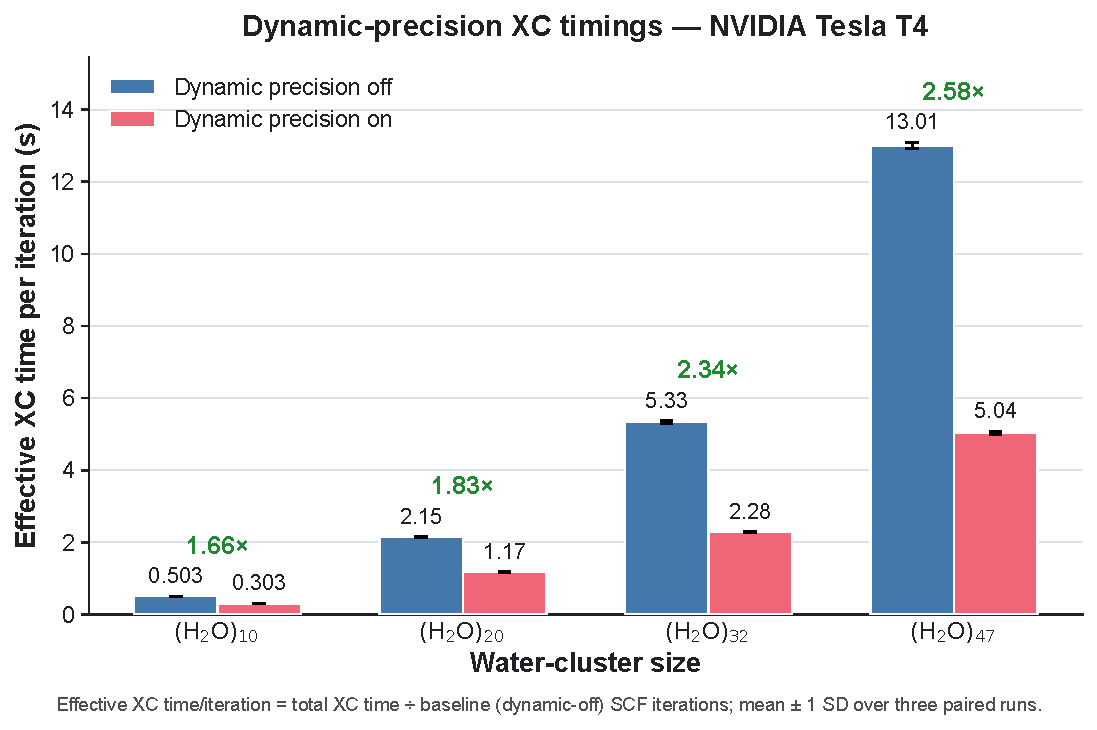
\includegraphics[width=0.96\linewidth]
    {Tesla_T4/dynamic_precision_xc_timings_T4.pdf}
  \caption{Effect of dynamic precision on XC timings for the NVIDIA Tesla T4.
  Effective XC time per iteration is the total XC time divided by the
  dynamic-off SCF iteration count of the corresponding paired run.  Bars show
  the mean over three paired runs, error bars denote $\pm 1$ sample standard
  deviation, and green labels give the mean effective XC speedup.}
  \label{fig:dynamic_precision_t4}
\end{figure}

\begin{figure}[htbp]
  \centering
  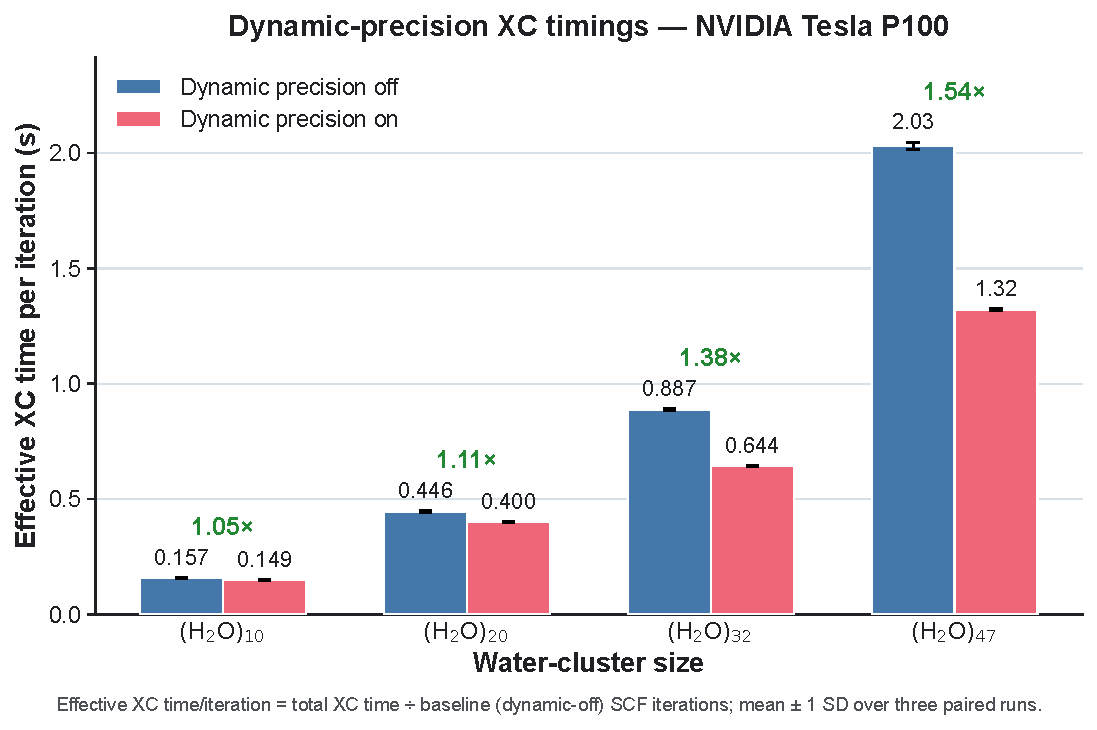
\includegraphics[width=0.96\linewidth]
    {P100/dynamic_precision_xc_timings_P100.pdf}
  \caption{Effect of dynamic precision on XC timings for the NVIDIA Tesla P100.
  The definition of the effective timing, averaging, error bars, and speedup
  labels is the same as in Figure~\ref{fig:dynamic_precision_t4}.}
  \label{fig:dynamic_precision_p100}
\end{figure}

\begin{table}[p]
\centering
\caption{Run-resolved Tesla T4 results.  Slash-separated entries are
dynamic precision off/on.  $\Delta E=E_{\mathrm{on}}-E_{\mathrm{off}}$ and
$t_{\mathrm{XC}}^{\mathrm{eff}}=T_{\mathrm{XC}}/N_{\mathrm{off}}$ for both
entries in that column.  All calculations converged.}
\label{tab:dynamic_precision_t4}
\setlength{\tabcolsep}{3.5pt}
\renewcommand{\arraystretch}{1.08}
\resizebox{\textwidth}{!}{%
\begin{tabular}{llrrrrrrr}
\toprule
System & Run &
\shortstack{$E_{\mathrm{off}}$\\($E_{\mathrm h}$)} &
\shortstack{$\Delta E$\\($10^{-8}E_{\mathrm h}$)} &
\shortstack{$N_{\mathrm{SCF}}$\\(off/on)} &
\shortstack{$T_{\mathrm{total}}$ (s)\\(off/on)} &
\shortstack{$T_{\mathrm{XC}}$ (s)\\(off/on)} &
\shortstack{$t_{\mathrm{XC}}^{\mathrm{eff}}$ (s)\\(off/on)} &
$S_{\mathrm{XC}}^{\mathrm{eff}}$ \\
\midrule
$(\mathrm{H_2O})_{10}$ & 1 & -762.860988885 & -0.584 & 22/24 & 19.55/15.68 & 11.08/6.81 & 0.504/0.310 & 1.627 \\
$(\mathrm{H_2O})_{10}$ & 2 & -762.860988885 & -0.584 & 22/24 & 19.13/14.83 & 11.21/6.57 & 0.510/0.299 & 1.706 \\
$(\mathrm{H_2O})_{10}$ & 3 & -762.860988885 & -0.584 & 22/24 & 19.00/14.99 & 10.91/6.61 & 0.496/0.300 & 1.651 \\
\addlinespace
$(\mathrm{H_2O})_{20}$ & 1 & -1525.790398809 & -12.866 & 21/24 & 74.77/56.15 & 44.98/24.80 & 2.142/1.181 & 1.814 \\
$(\mathrm{H_2O})_{20}$ & 2 & -1525.790398809 & -12.866 & 21/24 & 74.23/53.73 & 45.44/24.31 & 2.164/1.158 & 1.869 \\
$(\mathrm{H_2O})_{20}$ & 3 & -1525.790398809 & -12.866 & 21/24 & 73.29/54.46 & 44.87/24.80 & 2.137/1.181 & 1.809 \\
\addlinespace
$(\mathrm{H_2O})_{32}$ & 1 & -2441.350220620 & 1.473 & 34/32 & 270.44/166.41 & 181.76/77.82 & 5.346/2.289 & 2.336 \\
$(\mathrm{H_2O})_{32}$ & 2 & -2441.350220620 & 1.473 & 34/32 & 262.10/161.01 & 179.69/76.87 & 5.285/2.261 & 2.338 \\
$(\mathrm{H_2O})_{32}$ & 3 & -2441.350220620 & 1.472 & 34/32 & 268.25/161.79 & 182.30/78.11 & 5.362/2.297 & 2.334 \\
\addlinespace
$(\mathrm{H_2O})_{47}$ & 1 & -3585.736596697 & 0.369 & 27/27 & 565.92/354.51 & 351.67/136.35 & 13.025/5.050 & 2.579 \\
$(\mathrm{H_2O})_{47}$ & 2 & -3585.736596697 & 0.365 & 27/27 & 552.83/339.60 & 348.70/134.91 & 12.915/4.997 & 2.585 \\
$(\mathrm{H_2O})_{47}$ & 3 & -3585.736596697 & 0.369 & 27/27 & 559.98/344.38 & 353.44/137.18 & 13.090/5.081 & 2.576 \\
\bottomrule
\end{tabular}%
}
\end{table}

\begin{table}[p]
\centering
\caption{Run-resolved Tesla P100 results.  Definitions and slash-separated
off/on notation are the same as in Table~\ref{tab:dynamic_precision_t4}.
All calculations converged.}
\label{tab:dynamic_precision_p100}
\setlength{\tabcolsep}{3.5pt}
\renewcommand{\arraystretch}{1.08}
\resizebox{\textwidth}{!}{%
\begin{tabular}{llrrrrrrr}
\toprule
System & Run &
\shortstack{$E_{\mathrm{off}}$\\($E_{\mathrm h}$)} &
\shortstack{$\Delta E$\\($10^{-8}E_{\mathrm h}$)} &
\shortstack{$N_{\mathrm{SCF}}$\\(off/on)} &
\shortstack{$T_{\mathrm{total}}$ (s)\\(off/on)} &
\shortstack{$T_{\mathrm{XC}}$ (s)\\(off/on)} &
\shortstack{$t_{\mathrm{XC}}^{\mathrm{eff}}$ (s)\\(off/on)} &
$S_{\mathrm{XC}}^{\mathrm{eff}}$ \\
\midrule
$(\mathrm{H_2O})_{10}$ & 1 & -762.860988885 & -0.584 & 22/24 & 10.46/10.16 & 3.42/3.30 & 0.155/0.150 & 1.036 \\
$(\mathrm{H_2O})_{10}$ & 2 & -762.860988885 & -0.584 & 22/24 & 10.53/10.19 & 3.52/3.27 & 0.160/0.149 & 1.076 \\
$(\mathrm{H_2O})_{10}$ & 3 & -762.860988885 & -0.584 & 22/24 & 10.39/10.17 & 3.41/3.26 & 0.155/0.148 & 1.046 \\
\addlinespace
$(\mathrm{H_2O})_{20}$ & 1 & -1525.790398809 & -12.866 & 21/24 & 32.22/31.01 & 9.30/8.45 & 0.443/0.402 & 1.101 \\
$(\mathrm{H_2O})_{20}$ & 2 & -1525.790398809 & -12.867 & 21/24 & 32.72/31.02 & 9.46/8.41 & 0.450/0.400 & 1.125 \\
$(\mathrm{H_2O})_{20}$ & 3 & -1525.790398809 & -12.866 & 21/24 & 32.35/31.09 & 9.33/8.37 & 0.444/0.399 & 1.115 \\
\addlinespace
$(\mathrm{H_2O})_{32}$ & 1 & -2441.350220620 & 1.477 & 34/32 & 93.64/83.05 & 30.02/21.88 & 0.883/0.644 & 1.372 \\
$(\mathrm{H_2O})_{32}$ & 2 & -2441.350220620 & 1.478 & 34/32 & 94.33/83.94 & 30.32/21.96 & 0.892/0.646 & 1.381 \\
$(\mathrm{H_2O})_{32}$ & 3 & -2441.350220620 & 1.476 & 34/32 & 93.55/83.41 & 30.12/21.84 & 0.886/0.642 & 1.379 \\
\addlinespace
$(\mathrm{H_2O})_{47}$ & 1 & -3585.736596697 & -0.981 & 27/26 & 201.33/185.32 & 54.33/35.65 & 2.012/1.320 & 1.524 \\
$(\mathrm{H_2O})_{47}$ & 2 & -3585.736596697 & -0.983 & 27/26 & 204.07/186.04 & 55.19/35.64 & 2.044/1.320 & 1.549 \\
$(\mathrm{H_2O})_{47}$ & 3 & -3585.736596697 & -0.982 & 27/26 & 203.03/186.11 & 54.98/35.83 & 2.036/1.327 & 1.534 \\
\bottomrule
\end{tabular}%
}
\end{table}

\subsection{Results and interpretation}

Dynamic precision substantially reduced the XC cost on the Tesla T4
(Table~\ref{tab:dynamic_precision_t4}).  The
mean effective XC speedups were 1.66, 1.83, 2.34, and $2.58\times$ for
$(\mathrm{H_2O})_{10}$, $(\mathrm{H_2O})_{20}$,
$(\mathrm{H_2O})_{32}$, and $(\mathrm{H_2O})_{47}$, respectively.  These
correspond to mean reductions in accumulated XC time of 39.8\%, 45.4\%,
57.2\%, and 61.2\%.  The corresponding mean total-wall-time reductions were
21.1\%, 26.1\%, 38.9\%, and 38.1\%; these smaller end-to-end gains reflect
the non-XC portions of the calculation.

The benefit was smaller on the Tesla P100
(Table~\ref{tab:dynamic_precision_p100}): the effective XC speedups were
1.05, 1.11, 1.38, and $1.54\times$, corresponding to accumulated-XC-time
reductions of 5.0\%, 10.2\%, 27.4\%, and 34.9\%.  Mean total-wall-time
reductions were 2.7\%, 4.3\%, 11.1\%, and 8.4\%, respectively.  For the two
smallest clusters, the P100 per-cycle XC acceleration of approximately
$1.15$--$1.27\times$ was largely offset by the 2--3 additional SCF
iterations, leaving only $1.05$--$1.11\times$ effective speedup.

The SCF iteration changes were reproducible across all three runs.  Dynamic
precision required two and three additional iterations for
$(\mathrm{H_2O})_{10}$ and $(\mathrm{H_2O})_{20}$, respectively, but two
fewer iterations for $(\mathrm{H_2O})_{32}$.  For
$(\mathrm{H_2O})_{47}$, the iteration count was unchanged on the T4 and was
reduced by one on the P100.  The convergence-adjusted metric therefore
retains the penalty or benefit of these changes instead of masking them by
normalizing each mode by its own iteration count.  All calculations
converged, and the largest absolute difference between the final energies of
a paired dynamic-on and dynamic-off calculation was
$1.29\times10^{-7}\ E_{\mathrm h}$.

The stronger and increasingly favorable acceleration on the T4 is consistent
with its much larger fp32-to-fp64 throughput ratio (32:1) than that of the
P100 (2:1), as noted in the main text.  The P100 therefore gains relatively
little from using fp32 during the early iterations, particularly for the
small clusters where fixed and non-XC overheads are more prominent.  These
results show that dynamic precision is most advantageous on GPUs with a large
single- versus double-precision throughput disparity and when XC evaluation
constitutes a substantial fraction of the calculation.
